% This is "sig-alternate.tex" V2.1 April 2013
% This file should be compiled with V2.5 of "sig-alternate.cls" May 2012
%
% This example file demonstrates the use of the 'sig-alternate.cls'
% V2.5 LaTeX2e document class file. It is for those submitting
% articles to ACM Conference Proceedings WHO DO NOT WISH TO
% STRICTLY ADHERE TO THE SIGS (PUBS-BOARD-ENDORSED) STYLE.
% The 'sig-alternate.cls' file will produce a similar-looking,
% albeit, 'tighter' paper resulting in, invariably, fewer pages.
%
% ----------------------------------------------------------------------------------------------------------------
% This .tex file (and associated .cls V2.5) produces:
%       1) The Permission Statement
%       2) The Conference (location) Info information
%       3) The Copyright Line with ACM data
%       4) NO page numbers
%
% as against the acm_proc_article-sp.cls file which
% DOES NOT produce 1) thru' 3) above.
%
% Using 'sig-alternate.cls' you have control, however, from within
% the source .tex file, over both the CopyrightYear
% (defaulted to 200X) and the ACM Copyright Data
% (defaulted to X-XXXXX-XX-X/XX/XX).
% e.g.
% \CopyrightYear{2007} will cause 2007 to appear in the copyright line.
% \crdata{0-12345-67-8/90/12} will cause 0-12345-67-8/90/12 to appear in the copyright line.
%
% ---------------------------------------------------------------------------------------------------------------
% This .tex source is an example which *does* use
% the .bib file (from which the .bbl file % is produced).
% REMEMBER HOWEVER: After having produced the .bbl file,
% and prior to final submission, you *NEED* to 'insert'
% your .bbl file into your source .tex file so as to provide
% ONE 'self-contained' source file.
%
% ================= IF YOU HAVE QUESTIONS =======================
% Questions regarding the SIGS styles, SIGS policies and
% procedures, Conferences etc. should be sent to
% Adrienne Griscti (griscti@acm.org)
%
% Technical questions _only_ to
% Gerald Murray (murray@hq.acm.org)
% ===============================================================
%
% For tracking purposes - this is V2.0 - May 2012

\documentclass{sig-alternate-05-2015}
\usepackage{amsmath}
\usepackage{multirow}
\usepackage{natbib}
\usepackage{url}

\DeclareMathOperator*{\argmin}{\arg\!\min}
\DeclareMathOperator*{\argmax}{\arg\!\max}
\newcommand{\mat}[1]{\mathbf{#1}}


\begin{document}

% Copyright
\setcopyright{acmcopyright}
%\setcopyright{acmlicensed}
%\setcopyright{rightsretained}
%\setcopyright{usgov}
%\setcopyright{usgovmixed}
%\setcopyright{cagov}
%\setcopyright{cagovmixed}



% DOI
\doi{10.475/123_4}

% ISBN
\isbn{123-4567-24-567/08/06}

%Conference
\conferenceinfo{ACM Recsys '16}{Somewhen and somewhere}

\acmPrice{\$15.00}

%
% --- Author Metadata here ---
\conferenceinfo{WOODSTOCK}{'97 El Paso, Texas USA}
%\CopyrightYear{2007} % Allows default copyright year (20XX) to be over-ridden - IF NEED BE.
%\crdata{0-12345-67-8/90/01}  % Allows default copyright data (0-89791-88-6/97/05) to be over-ridden - IF NEED BE.
% --- End of Author Metadata ---

\title{Deep Learning for Long-term Dependencies in Sequential Recommendation}
%\subtitle{[Extended Abstract]
%\titlenote{A full version of this paper is available as
%\textit{Author's Guide to Preparing ACM SIG Proceedings Using
%\LaTeX$2_\epsilon$\ and BibTeX} at
%\texttt{www.acm.org/eaddress.htm}}}


%
% You need the command \numberofauthors to handle the 'placement
% and alignment' of the authors beneath the title.
%
% For aesthetic reasons, we recommend 'three authors at a time'
% i.e. three 'name/affiliation blocks' be placed beneath the title.
%
% NOTE: You are NOT restricted in how many 'rows' of
% "name/affiliations" may appear. We just ask that you restrict
% the number of 'columns' to three.
%
% Because of the available 'opening page real-estate'
% we ask you to refrain from putting more than six authors
% (two rows with three columns) beneath the article title.
% More than six makes the first-page appear very cluttered indeed.
%
% Use the \alignauthor commands to handle the names
% and affiliations for an 'aesthetic maximum' of six authors.
% Add names, affiliations, addresses for
% the seventh etc. author(s) as the argument for the
% \additionalauthors command.
% These 'additional authors' will be output/set for you
% without further effort on your part as the last section in
% the body of your article BEFORE References or any Appendices.

\numberofauthors{2} %  in this sample file, there are a *total*
% of EIGHT authors. SIX appear on the 'first-page' (for formatting
% reasons) and the remaining two appear in the \additionalauthors section.
%
\author{
% You can go ahead and credit any number of authors here,
% e.g. one 'row of three' or two rows (consisting of one row of three
% and a second row of one, two or three).
%
% The command \alignauthor (no curly braces needed) should
% precede each author name, affiliation/snail-mail address and
% e-mail address. Additionally, tag each line of
% affiliation/address with \affaddr, and tag the
% e-mail address with \email.
%
% 1st. author
\alignauthor
Harold Soh\\
       \affaddr{University of Toronto}\\
       \email{harold.soh@utoronto.ca}
% 2nd. author
\alignauthor
Scott Sanner\\
       \affaddr{University of Toronto}\\
       \email{scott.sanner@utoronto.ca}
%% 3rd. author
%\alignauthor Lars Th{\o}rv{\"a}ld\titlenote{This author is the
%one who did all the really hard work.}\\
%       \affaddr{The Th{\o}rv{\"a}ld Group}\\
%       \affaddr{1 Th{\o}rv{\"a}ld Circle}\\
%       \affaddr{Hekla, Iceland}\\
%       \email{larst@affiliation.org}
%\and  % use '\and' if you need 'another row' of author names
%% 4th. author
%\alignauthor Lawrence P. Leipuner\\
%       \affaddr{Brookhaven Laboratories}\\
%       \affaddr{Brookhaven National Lab}\\
%       \affaddr{P.O. Box 5000}\\
%       \email{lleipuner@researchlabs.org}
%% 5th. author
%\alignauthor Sean Fogarty\\
%       \affaddr{NASA Ames Research Center}\\
%       \affaddr{Moffett Field}\\
%       \affaddr{California 94035}\\
%       \email{fogartys@amesres.org}
%% 6th. author
%\alignauthor Charles Palmer\\
%       \affaddr{Palmer Research Laboratories}\\
%       \affaddr{8600 Datapoint Drive}\\
%       \affaddr{San Antonio, Texas 78229}\\
%       \email{cpalmer@prl.com}
}
% There's nothing stopping you putting the seventh, eighth, etc.
% author on the opening page (as the 'third row') but we ask,
% for aesthetic reasons that you place these 'additional authors'
% in the \additional authors block, viz.
%\additionalauthors{Additional authors: John Smith (The Th{\o}rv{\"a}ld Group,
%email: {\texttt{jsmith@affiliation.org}}) and Julius P.~Kumquat
%(The Kumquat Consortium, email: {\texttt{jpkumquat@consortium.net}}).}
\date{30 July 1999}
% Just remember to make sure that the TOTAL number of authors
% is the number that will appear on the first page PLUS the
% number that will appear in the \additionalauthors section.

\maketitle
\begin{abstract}
Real-world recommender systems are often required to make predictions not just of individual items but rather sequences. For example, retails products are suggested based on past transactions, and relevant websites on viewing histories. Existing sequential recommendation methods, i.e., Markov chain (MC) models and tensor-factorized versions, are constructed under the Markov assumption, which is untenable in many practical applications. In this paper, we propose and evaluate a deep learning model for sequential item recommendation that uses gated recurrent memory cells to capture long-term dependencies. Consequently, the model constructs embedding contexts that jointly capture user characteristics and purchase/rating histories. In a comparative evaluation over  datasets in web and education, we demonstrate that the non-Markovian aspect of our model results in improved novel item recommendations.  
\end{abstract}


%
% The code below should be generated by the tool at
% http://dl.acm.org/ccs.cfm
% Please copy and paste the code instead of the example below. 
%
\begin{CCSXML}
<ccs2012>
 <concept>
  <concept_id>10010520.10010553.10010562</concept_id>
  <concept_desc>Computer systems organization~Embedded systems</concept_desc>
  <concept_significance>500</concept_significance>
 </concept>
 <concept>
  <concept_id>10010520.10010575.10010755</concept_id>
  <concept_desc>Computer systems organization~Redundancy</concept_desc>
  <concept_significance>300</concept_significance>
 </concept>
 <concept>
  <concept_id>10010520.10010553.10010554</concept_id>
  <concept_desc>Computer systems organization~Robotics</concept_desc>
  <concept_significance>100</concept_significance>
 </concept>
 <concept>
  <concept_id>10003033.10003083.10003095</concept_id>
  <concept_desc>Networks~Network reliability</concept_desc>
  <concept_significance>100</concept_significance>
 </concept>
</ccs2012>  
\end{CCSXML}

\ccsdesc[500]{Computer systems organization~Embedded systems}
\ccsdesc[300]{Computer systems organization~Redundancy}
\ccsdesc{Computer systems organization~Robotics}
\ccsdesc[100]{Networks~Network reliability}


%
% End generated code
%

%
%  Use this command to print the description
%
\printccsdesc

% We no longer use \terms command
%\terms{Theory}

\keywords{Collaborative Filtering; Sequential Recommendation; Bayesian Model Averaging}

\section{Introduction}
\paragraph{Why is Sequential recommendation is important? examples?}


\paragraph{Existing methods?} 
\begin{itemize}
\item Tensor factorization: non-convex, requires tuning (hyperparameters, latent dimensionality), difficult for online use.
\item Nearest Neighbor methods via specialized similarity scores for time series: ad-hoc similarity scores, 
\end{itemize}

\paragraph{Our contributions?}


\paragraph{How is it novel?} 

\paragraph{Main messages?}

\paragraph{Paper organization?}


\section{Background and Related Work}
What is the formal definition of the work?

What existing methods are there?
\begin{itemize}
\item Rendle, S., Freudenthaler, C., Schmidt-Thieme, L. (2010). Factorizing personalized Markov chains for next-basket recommendation. Proceedings of the 19th International Conference on World Wide Web - WWW'10, 811.
\item Feng, S., Li, X., Zeng, Y., Cong, G., Chee, Y. M., Yuan, Q. (2015). Personalized Ranking Metric Embedding for Next New POI Recommendation. IJCAI International Joint Conference on Artificial Intelligence, (IJCAI), 2069-2075.
\item Yap, G. E., Li, X. L., Yu, P. S. (2012). Effective next-items recommendation via personalized sequential pattern mining. Lecture Notes in Computer Science (Including Subseries Lecture Notes in Artificial Intelligence and Lecture Notes in Bioinformatics), 7239 LNCS(PART 2), 48-64.
\item Cheng, C., Yang, H., Lyu, M. R., King, I. (2013). Where you like to go next: Successive point-of-interest recommendation. IJCAI International Joint Conference on Artificial Intelligence, 2605-2611.
\end{itemize}
 
\section{Deep Sequential Recommendation}

Problem formulation. Challenges when applying deep learning. Large itemsets. 

\subsection{Model Architecture}

\begin{figure}
\centering
	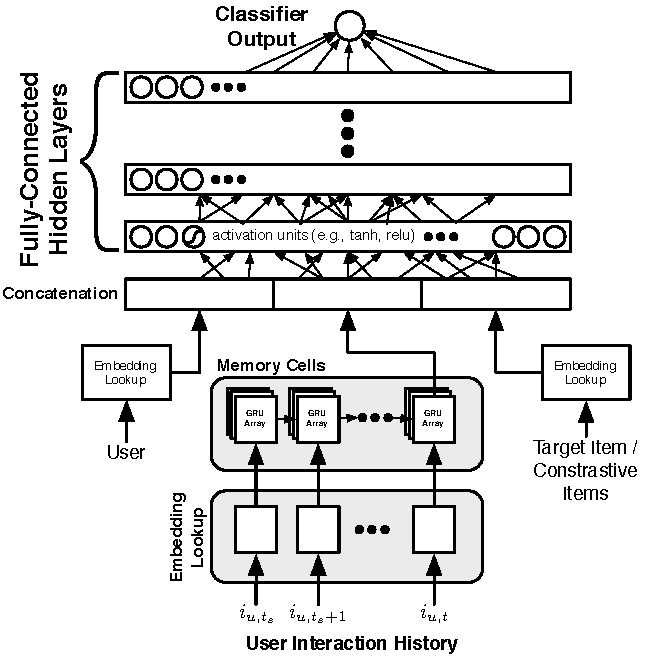
\includegraphics[width=7cm]{images/ModelArch}
	\caption{Model Architecture for Deep Sequential Recommendation. At a high-level, the model comprises three basic component layers responsible for (i) encoding the input as real vectors (embeddings), (ii) compressing the input sequence as a ``memory state'', and (iii) making a final selection/ranking of next items to be recommended (hidden layers and classifier). The entire model is trained via back-propagation using candidate sampling. See text for details.}
	\label{fig:ModelArch}
\end{figure}

A high-level overview of our model architecture is shown in Fig. \ref{fig:ModelArch}. 

\subsection{Memory: Gated Recurrent Units}
\begin{figure}
\centering
	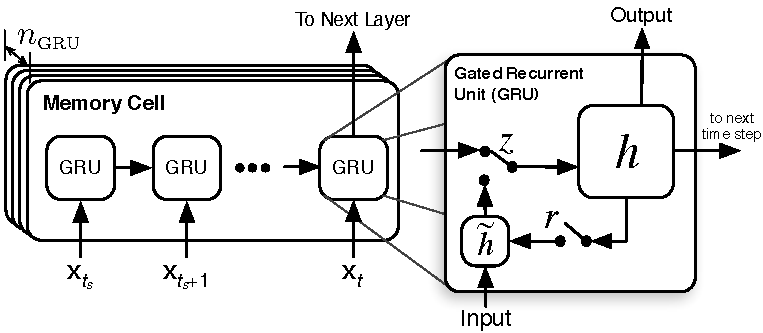
\includegraphics[width=8cm]{images/GRU}
	\caption{The model's memory is composed of Gated Recurrent Units (GRU) cells that selectively update or reset their hidden states via two gates. An interaction history is fed an item at a time into the cell and the update gate $z$ determines whether the internal state $h$ is replaced by a new hidden state $\tilde{h}$. The reset gate $r$ controls whether to disregard the previous hidden state. Although sometimes shown as discrete gates (as above), the updates/resets are weighted averages using parameters learnt from data. After the history is fed, and the final state is relayed to higher layers. See text for  details. }
	\label{fig:GRU}
\end{figure}

In our model, we use the Gated Recurrent Unit (GRU)~\cite{Cho2014} (Fig. \ref{fig:GRU}), a streamlined variant of Long Short-Term Memory (LSTM)~\cite{Hochreiter1997}, that has become increasingly popular due to its simplicity and performance~\cite{jozefowicz2015empirical}. In traditional RNN models, a cell lacked control over the evolution of its hidden state. In contrast, the GRU learns to operate two internal structures---the update and reset gates---that allow it to control what to remember and forget. More formally, consider that a cell $j$ has state $h_{t-1}^{(j)}$ and receives a new input $\mathbf{x}_t$. The cell's updated internal state is given by
\begin{align}
	h_t^{(j)} = (1-z_t^{(j)})h^{(j)}_{t-1} + z_t^{(j)}\tilde{h}_{t}^{(j)},
\end{align}
which is a weighted average of its previous state and a  candidate activation $\tilde{h}_{t}^{(j)}$. This interpolation is controlled by the update gate $z_t^{(j)}$, which relies on two learnt parameters $\mat{W}_z$ and $\mat{U}_z$,
\begin{align}
	z_t^{(j)} = \textrm{sigm}\big([\mat{W}_z\mat{x}_{t} + \mat{U}_z\mat{h}_{t-1})]_j\big).
\end{align}
The candidate activation $\tilde{h}_{t}^{(j)}$ is computed via
\begin{align}
	\tilde{h}_{t}^{(j)} = \mathrm{tanh}([\mat{W}\mat{x}_t + \mat{U}(\mat{r}_t \odot \mat{h}_{t-1})]_j )
\end{align}
where $\odot$ denotes element-wise multiplication. The cell's reset gate $r^{(j)}_t = [\mat{r}_t]_j$ is also determined by two learnt matrices $\mat{W}_r$ and $\mat{U}_r$,
\begin{align}
	r^{(j)}_t = \textrm{sigm}\big([\mat{W}_r\mat{x}_{t} + \mat{U}_r\mat{h}_{t-1})]_j\big)
\end{align}
The previous hidden state is effectively dropped when the reset gate's value nears zero, and as such, cells that learn short-term dependencies will have active reset gates. In comparison, cells that learn to model long-term dependencies will have active update gates~\cite{Cho2014}. 

   
\subsection{Training via Candidate Sampling}
Given a user $u$ and previous interactions $a_{u,t}$, we would like to train our model to recommend an item $i \in I$. Adopting the classification perspective allows us to train our model via backpropagation using standard techniques. However, this approach is complicated by large item sets $I$ common in recommendation settings; it becomes infeasible to compute typical loss functions, such as the softmax and logistic losses. 

To address this problem, we use a technique termed as \emph{candidate sampling}~\cite{TFCandidateSampling} whereby the loss is evaluated against a small set of candidate or contrastive classes instead of over the entire set $I$. In our preliminary experiments, the sampled softmax~\cite{Jean2015} worked best (compared to Noise Contrastive Estimation and the sampled logistic) and is given by
\begin{align}
	\mathcal{L}_{\textsc{sm}}
\end{align}

Given our context $x_{u,t} = (u, h_{u,t})$, we would like to train our model to predict relative log probabilities of an item, $F(x,y) = \log p(y|x_{u,t}) + C(x) \propto \log p(y|x_{u,t})$ where $C(x)$ does not depend on $y$. The canonical log softmax loss is given by:
\begin{align}
	\mathcal{L}_{\textsc{sm}} = \sum_j -H(x_{u,t}, i_{t+1}) + \log \left( \sum_{i'} \exp H(x_{u,t}, i') \right)
\end{align}
where 


\section{Experiments}
In this section, we report on experiments comparing the DRNN to a baseline Markov chain (MC) and the tensor Factorized Personalized Markov Chain (FPMC) models~\cite{Rendle2010}. In addition, we constructed a deep neural network (DNN) identical to the DRNN, but without the memory cells; this allowed us to isolate the effect of capturing temporal dependencies greater than the first-order on the quality of recommendations.

\subsection{Experimental Setup}
We adopt the experimental setup outlined in \cite{Rendle2010}; given the interaction history, our methods were tasked to predict the last \emph{unique} item in the sequence. We used two moderately-sized datasets: the Microsoft Web (MSWeb) and the Assistments'15 educational datasets. Following \cite{Rendle2010}, users that did not interact with at least 10 items were dropped. 

To test the variability of the methods under slightly different conditions, we performed a variant of 10-fold cross-validation where 90\% of the \emph{last} items were used for testing and 10\% for validation. Early stopping was used when training FPMC, DNN and DRNN, whereby training was halted with the HLU computed on the validation set did not improve after 1000 positive training samples. A maximum of $2\times 10^6$ iterations was permitted for FPMC, and $2\times 10^5$ iterations (100-sample mini-batches) for both DNN and DRNN. 

As performance scores, we computed four standard metrics: the Breese score or Half-Life Utility (HLU), Top-5 F1, precision, and recall. 



\subsection{Performance Results}
\begin{figure}
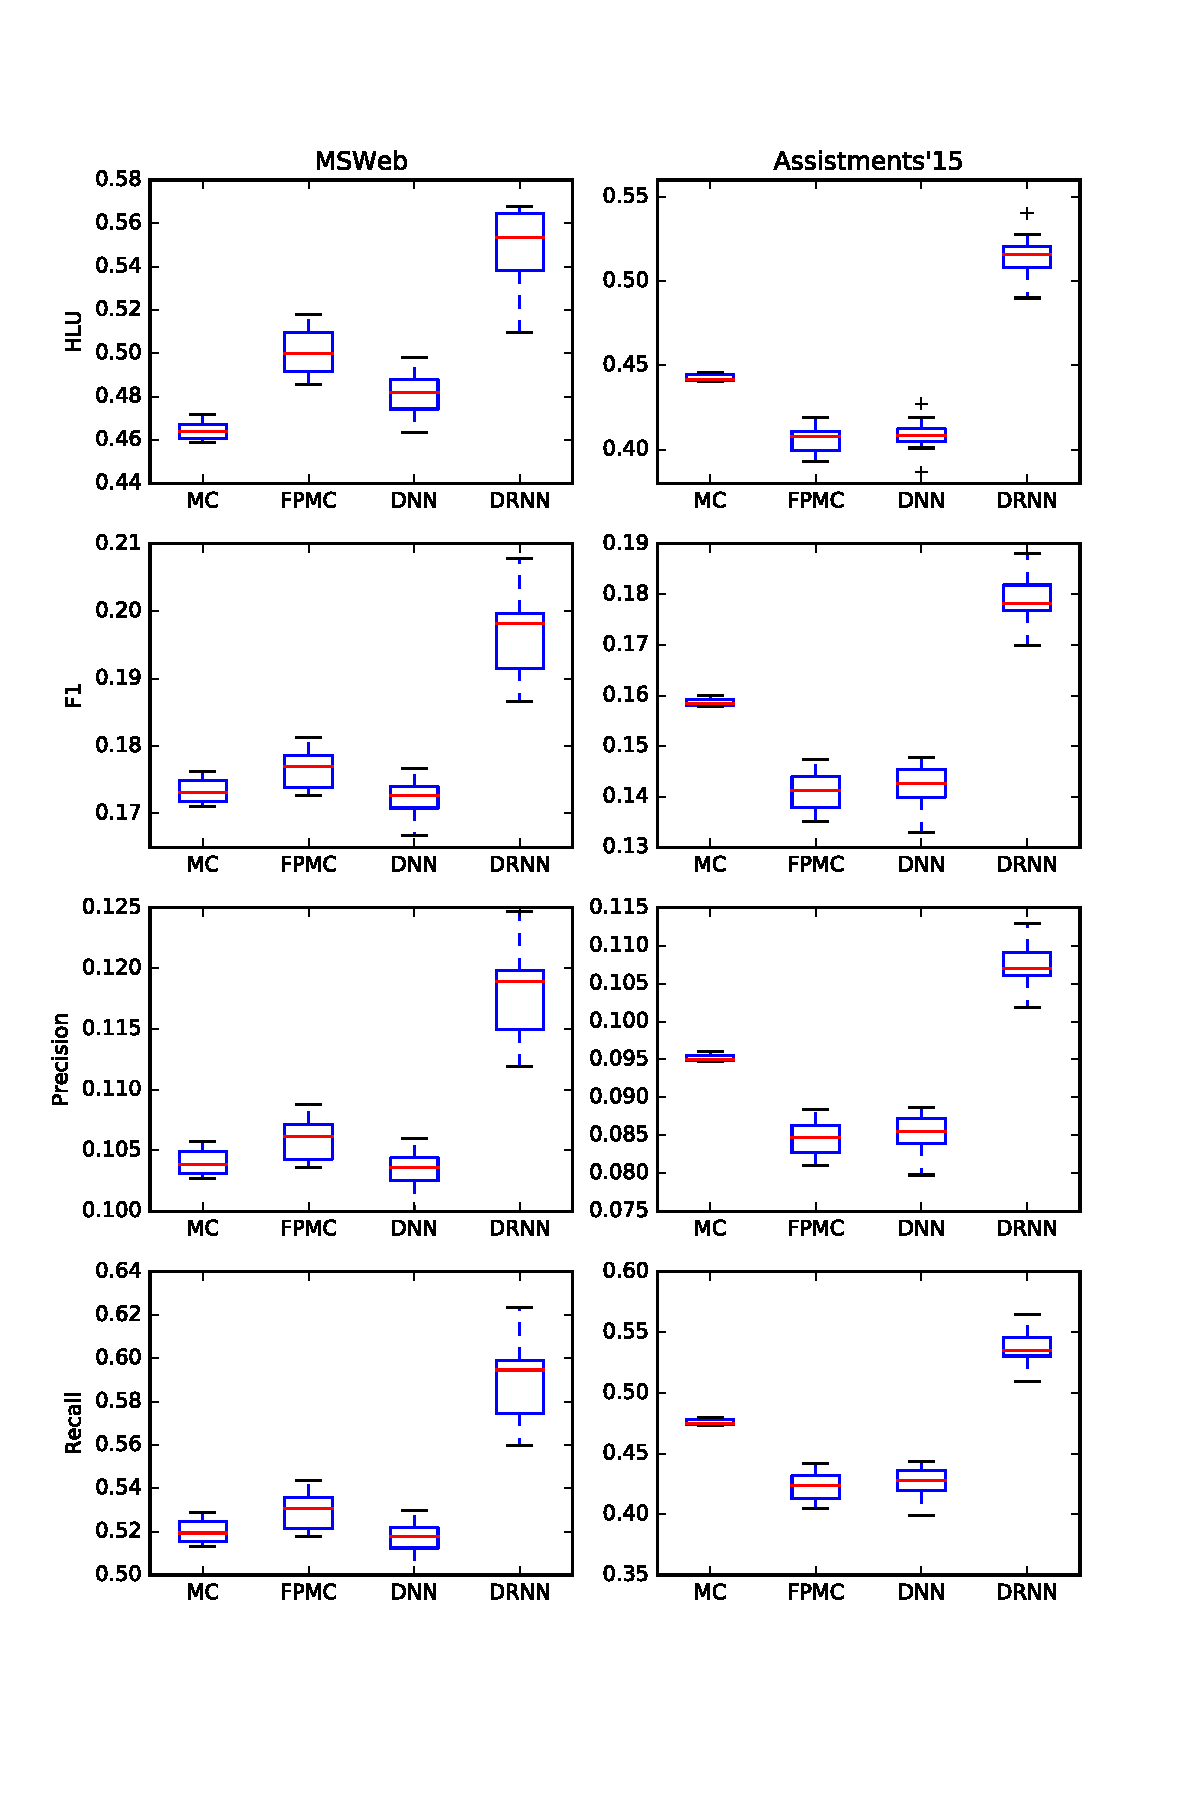
\includegraphics[width=8cm]{images/PerfBoxplots}		
\caption{Performance scores on the MSWeb and Assistments'15 datasets. In both datasets, the DRNN achieves the best scores,  suggesting the importance of long-term dependencies for the sequential recommendation task.}
\label{fig:PerfResults}
\end{figure}
Summarized scores achieved by the compared methods are shown in Fig. \ref{fig:PerfResults}.

\subsection{Embedding Size Effects}

\subsection{Length of Sequences}

%
%\begin{table}
%\begin{center} 
%\begin{tabular}{ |l|l|c|c|c|c|}
%\hline
%\multirow{2}{*}{\textbf{Dataset}} & \multirow{2}{*}{\textbf{Score}} & \multicolumn{4}{ |c| }{\textbf{Method}} \\  \cline{3-6}
%& & \textbf{MC} & \textbf{FPMC} & \textbf{ANN} & \textbf{LSTM} \\
%\hline
% \multirow{4}{*}{gowalla} 
% & HLU & \textbf{0.160} & 0.133 & 0.130 & 0.051 \\
% & Prec & \textbf{0.033} & 0.025  & 0.027 & 0.013 \\
% & Rec & \textbf{0.166} & 0.124 & 0.136 &  0.066 \\
% & F1 & \textbf{0.055} & 0.041 & 0.045 & 0.022 \\
% \hline
% \multirow{4}{*}{msweb} 
% & HLU & 0.485  & 0.522  & 0.489 & \textbf{0.566} \\
% & Prec & 0.107 & 0.109 & 0.106 & \textbf{0.124} \\
% & Rec & 0.537 & 0.546 & 0.528 & \textbf{0.621} \\
% & F1 & 0.179 & 0.182 & 0.176 & \textbf{0.207} \\
% \hline
% \multirow{4}{*}{assist15} 
% & HLU & 0.440 & 0.438  & 0.412 & \textbf{0.535} \\
% & Prec & 0.094 & 0.092  & 0.086 & \textbf{0.113} \\
% & Rec & 0.471 & 0.458  & 0.458 & \textbf{0.568} \\
% & F1 & 0.157 & 0.153 & 0.430 & \textbf{0.189} \\
% \hline
%\hline
%\end{tabular}
%\caption{Novel Item Recommendation}
%\end{center} 
%\end{table}


%
%\begin{table}
%\begin{center} 
%\caption{User Split Test}
%\begin{tabular}{ |l|l|c|c|c|}
%\hline
%\multirow{2}{*}{\textbf{Dataset}} & \multirow{2}{*}{\textbf{Score}} & \multicolumn{3}{ |c| }{\textbf{Method}} \\  \cline{3-5}
%& & \textbf{MC} & \textbf{BMA} & \textbf{BMA-Gb} \\
%\hline
% \multirow{4}{*}{gowalla} 
% & hlu & 0.160 & 0.162 & \textbf{0.165} \\
% & prec & 0.035 & 0.035 & \textbf{0.036 }\\
% & rec & 0.174 & 0.176 & \textbf{0.181} \\
% & f1 & 0.058 & 0.059 & \textbf{0.060} \\
% \hline
% \multirow{4}{*}{msweb} 
%  & hlu & 0.541 & \textbf{0.545} & 0.540 \\
% & prec & 0.116 & \textbf{0.116} & 0.115 \\
% & rec & 0.581 & \textbf{0.582} & 0.577 \\
% & f1 & 0.194 & \textbf{0.194} & 0.192 \\
% \hline
% \multirow{4}{*}{assist15} 
% & hlu & 0.372 & \textbf{0.453} & 0.375 \\
% & prec & 0.076 & \textbf{0.095} & 0.077 \\
% & rec & 0.381 & \textbf{0.473} & 0.383 \\
% & f1 & 0.127 & \textbf{0.158} & 0.128 \\
% \hline
%%  \multirow{4}{*}{retail} 
%% & HLU & 0.005  & 0.019 & -1.000 \\
%% & Prec & 0.005  & 0.007 & -1.000 \\
%% & Rec & 0.004  & 0.015 & -1.000 \\
%% & F1 & 0.004  & 0.010 & -1.000 \\
%% \hline
%\hline
%\end{tabular}
%\end{center} 
%\end{table}

\subsection{Large Scale Experiment}
Need a Large Scale Experiment here! 


\section{Discussion}
Potential Extensions

\section{Summary and Conclusions}


%ACKNOWLEDGMENTS are optional
%\section{Acknowledgments}
%This section is optional; it is a location for you
%to acknowledge grants, funding, editing assistance and
%what have you.  In the present case, for example, the
%authors would like to thank Gerald Murray of ACM for
%his help in codifying this \textit{Author's Guide}
%and the \textbf{.cls} and \textbf{.tex} files that it describes.

%
% The following two commands are all you need in the
% initial runs of your .tex file to
% produce the bibliography for the citations in your paper.
\bibliographystyle{abbrv}
\bibliography{DeepSeqRec_Recsys16}  % sigproc.bib is the name of the Bibliography in this case
% You must have a proper ".bib" file
%  and remember to run:
% latex bibtex latex latex
% to resolve all references
%
% ACM needs 'a single self-contained file'!
%
%APPENDICES are optional
%\balancecolumns
%\appendix
%%Appendix A
%\section{Headings in Appendices}
%The rules about hierarchical headings discussed above for
%the body of the article are different in the appendices.
%In the \textbf{appendix} environment, the command
%\textbf{section} is used to
%indicate the start of each Appendix, with alphabetic order
%designation (i.e. the first is A, the second B, etc.) and
%a title (if you include one).  So, if you need
%hierarchical structure
%\textit{within} an Appendix, start with \textbf{subsection} as the
%highest level. Here is an outline of the body of this
%document in Appendix-appropriate form:
%\subsection{Introduction}
%\subsection{The Body of the Paper}
%\subsubsection{Type Changes and  Special Characters}
%\subsubsection{Math Equations}
%\paragraph{Inline (In-text) Equations}
%\paragraph{Display Equations}
%\subsubsection{Citations}
%\subsubsection{Tables}
%\subsubsection{Figures}
%\subsubsection{Theorem-like Constructs}
%\subsubsection*{A Caveat for the \TeX\ Expert}
%\subsection{Conclusions}
%\subsection{Acknowledgments}
%\subsection{Additional Authors}
%This section is inserted by \LaTeX; you do not insert it.
%You just add the names and information in the
%\texttt{{\char'134}additionalauthors} command at the start
%of the document.
%\subsection{References}
%Generated by bibtex from your ~.bib file.  Run latex,
%then bibtex, then latex twice (to resolve references)
%to create the ~.bbl file.  Insert that ~.bbl file into
%the .tex source file and comment out
%the command \texttt{{\char'134}thebibliography}.
%% This next section command marks the start of
%% Appendix B, and does not continue the present hierarchy
%\section{More Help for the Hardy}
%The sig-alternate.cls file itself is chock-full of succinct
%and helpful comments.  If you consider yourself a moderately
%experienced to expert user of \LaTeX, you may find reading
%it useful but please remember not to change it.
%\balancecolumns % GM June 2007
% That's all folks!
\end{document}
